\begin{definition}
    Let $(G,\lambda)$ be a graph over edge label set $\Sigma_E$.
    We define the signature $\Sigma$ of the hypergraph as
    $(\{\epsilon\}, \Sigma_E, \text{Type})$ where $\text{Type}(l) = \{\epsilon\epsilon\}$ for all $l \in \Sigma_E$. 
    Furthermore, we define $|(G,\lambda)|$ as the hypergraph $(V_G, E_G,\opn{mark}, \opn{lab},\text{att})$ over the signature $\Sigma$ where
    \begin{itemize}
        \item $\opn{mark}(v) = \epsilon$ for all $v \in V_G$,
        \item $\opn{lab}(e) = \lambda(e)$ for all $e \in E_G$,
        \item $\text{att}(e) = st \in V_G^*$ for all $e \in E_G$ with source $s$ and target $t$,
    \end{itemize}
\end{definition}

\begin{example}
    We show a graph $G$, on the left,and its hypergraph $|G|$,on the right.

    \begin{tikzpicture}[scale=0.75]
        \node[draw,circle] (l1) at (-3,3) {1};
        \node[draw,circle] (l2) at (3 ,3) {2};
        \node[draw,circle] (l3) at (0,0) {3};
        \draw[->] (l1) -- (l3) node[midway,left] {s};
        \draw[->] (l2) -- (l3) node[midway,right] {s};
        \draw[->] (l3) edge [loop below] node {0} (l3);
    \end{tikzpicture}
    \hspace{1cm}
    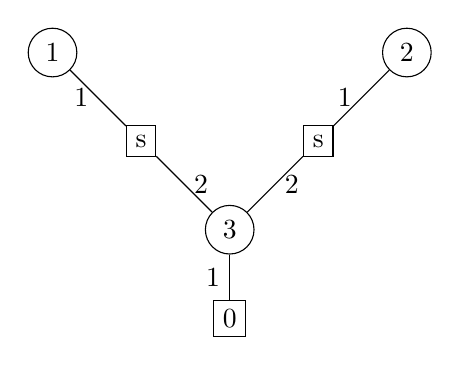
\begin{tikzpicture}[scale=0.75]
        \node[draw,circle] (n1) at (-3,3) {1};
        \node[draw,circle] (n2) at (3,3) {2};
        \node[draw,circle] (n3) at (0,0) {3};
        \node[draw,rectangle] (e1) at (-1.5,1.5) {s};
        \node[draw,rectangle] (e2) at (1.5,1.5) {s};
        \node[draw,rectangle] (e3) at (0, -1.5) {0};
        \draw (e1) -- (n1) node[midway,left] {1};
        \draw (e1) -- (n3) node[midway,right] {2};
        \draw (e2) -- (n2) node[midway,left] {1};
        \draw (e2) -- (n3) node[midway,right] {2};
        \draw (e3) -- (n3) node[midway,left] {1};
    \end{tikzpicture}
\end{example}

Since a graph homomorphism is a hypergraph homomorphism, we transform graph homomorphisms into hypergraph homomorphisms in a trivial way.
\begin{definition}
    Let $h: A \rightarrowtail B$ be a graph homomorphism. We define the hypergraph homomorphism $|h| : |A| \rightarrowtail |B|$ such that for all $v \in V_A$, $|h|(v) = h(v)$, for all $e \in E_A$, $|h|(e) = h(e)$.
\end{definition}

\begin{definition}
    Let $\rho = (L \overset{l}{\leftarrowtail} K \overset{r}{\rightarrowtail} R)$ be a DPO graph relabeling rule. We define the hypergraph rewriting rule $|\rho|$ as $|L| \overset{|l|}{\leftarrowtail} |K| \overset{|r|}{\rightarrowtail} |R|$. 
\end{definition}


\begin{theorem}
    Let $\rho$ be a DPO graph rewriting rule.
    For any DPO rewriting step from a graph $G$ to a graph $H$ using the rule $\rho$, there is a DPO hypergraph rewriting step from $|G|$ to $|H|$ using the rule $|\rho|$.
\end{theorem}
The proof is straightforward by definition.